% ---	
% primeiro capitulo de Resultados
% ---
\chapter{Apresentação e Análise dos Resultados}

Para medição dos tempos e comparações das implementações demonstradas na seção anterior, foi utilizado um computador pessoal de processador não-dedicado, modelo Intel® Core i7-7500U (3M Cache, 2.7 GHz até 3.5 GHz com Max Turbo). Os algoritmos foram executados no sistema operacional Ubuntu 18.04 e os resultados adicionados aos final dos respectivos arquivos na pasta outputs. 

Os tempos foram medidos tomando como referência somente a função de ordenação, de forma a evitar influência de possíveis \textit{overheads} de geração, entrada ou saída de dados. Alguns cenários, como Insertion Sort, para 1 milhão de entradas, não foram executados em 10 repetições por questões de tempo hábil, já que esses cenários demandavam muitas horas de execução.

Os gráficos para visualização dos dados gerados foram utilizados com o auxílio da biblioteca \textit{matplotlib} do python. O script para leitura e plotagem dos dados se encontra disponível junto ao código fonte. O mesmo pode ser executado no formato \textit{python charts.py |ASC|DESC||}, apenas com o parâmetro da ordenação a ser considerado, seguindo o mesmo padrão anterior. O código faz a leitura dos arquivos emitidos na execução, fazendo a média dos dados nas linhas presentes.

O primeiro resultado apresentado para os 3 algoritmos é dado pelas entradas em que os elementos estavam arranjados aleatoriamente. Neste caso, conforme mostra o gráfico, o algoritmo do Insertion Sort tende a fazer um elevado número de trocas e consequentemente se mostra mais lento que o Merge Sort e Tim Sort, que na escala visual se mostram bem próximos principalmente devido à diferença de ordem de seus resultados com o Insertion Sort. Mesmo nos piores cenários, os dois últimos não chegaram a demandar 10 segundos para execução, portanto, serão analisados de forma isolada posteriormente.


\begin{figure}[!htb]
\centering
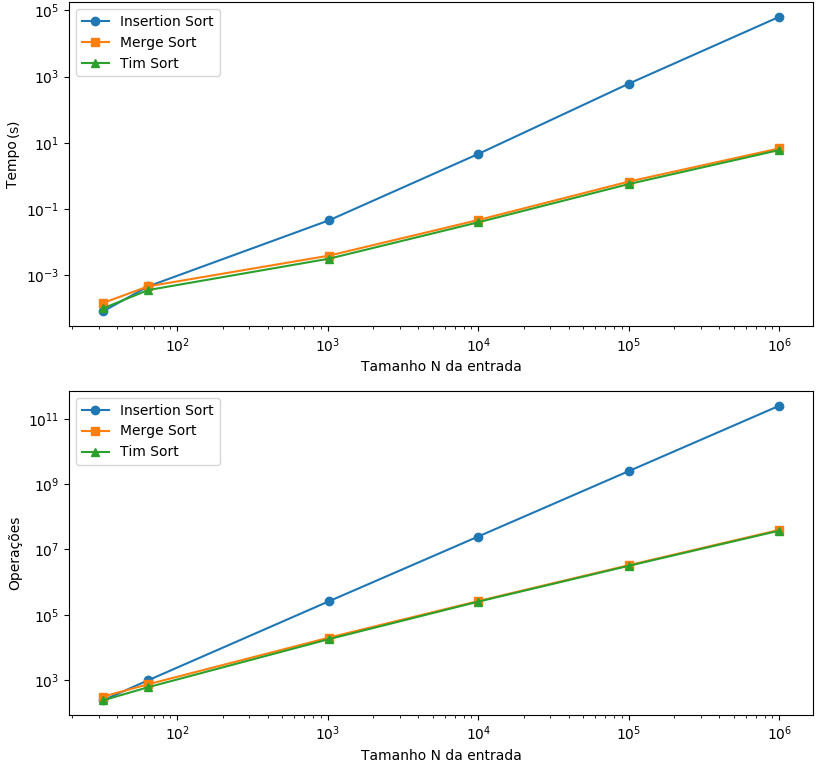
\includegraphics[width=15cm]{img/graficos_random.png}
\caption{Resultados de execução para entrada aleatória}
\label{fig:grafico_random}
\end{figure}

No segundo cenário, todavia, é o caso em que o Insertion Sort tem seu melhor caso (O(n)) e melhor performance dentre os 3 algoritmos. Como todos os elementos estão em ordem, na prática, o Insertion Sort faz apenas uma varredura no vetor verificando e nenhuma troca é efetuada. O Tim Sort por sua vez tende a performar melhor do que o Merge Sort, já que utiliza o Insertion Sort para ordenação das sub-listas e, portanto, esse cenário também o favorece.

\begin{figure}[!htb]
\centering
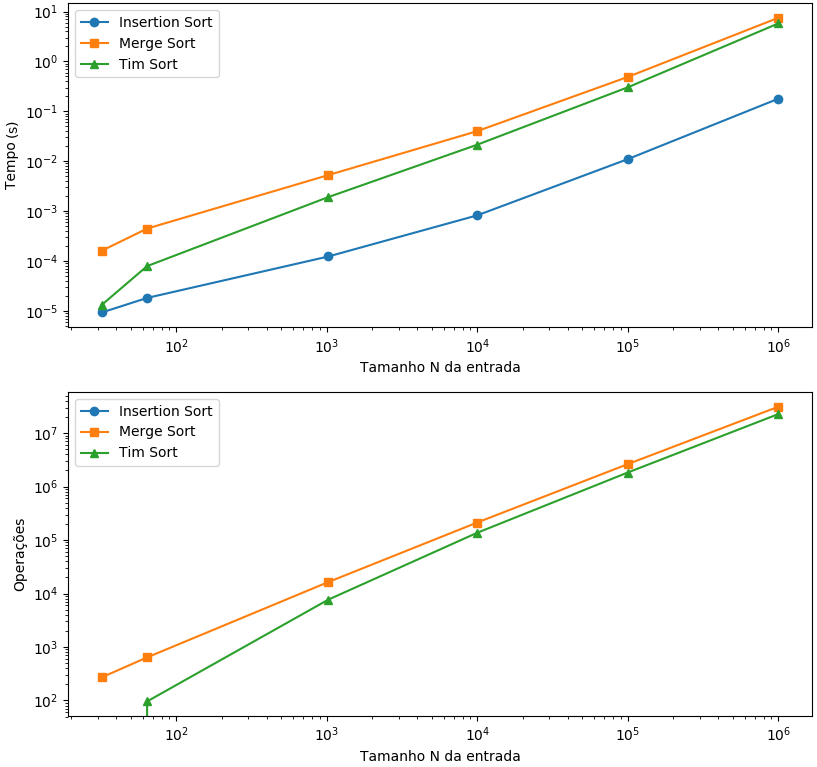
\includegraphics[width=15cm]{img/graficos_asc.png}
\caption{Resultados de execução para entrada ordenada crescentemente}
\label{fig:grafico_asc}
\end{figure}

Na última configuração de entrada, onde os elementos estão ordenados decrescentemente, o Insertion Sort encontra seu pior caso, O(n\textsuperscript{2}). Um detalhe importante a ser observado sobre o Tim Sort é que, apesar de utilizar o Insertion Sort, devido à sua estratégia de sub-divisão, o algoritmo ainda tem uma boa performance, bem próximo ao Merge Sort. Outra observação é que, apesar do tempo cerca de 2 vezes maior em relação à entrada aleatória, o traçado dos gráficos são bem semelhantes devido à escala logarítimica que se mostrou uma melhor escolha em razão do crescimento muito rápido da curva do Insertion Sort.

\begin{figure}[!htb]
\centering
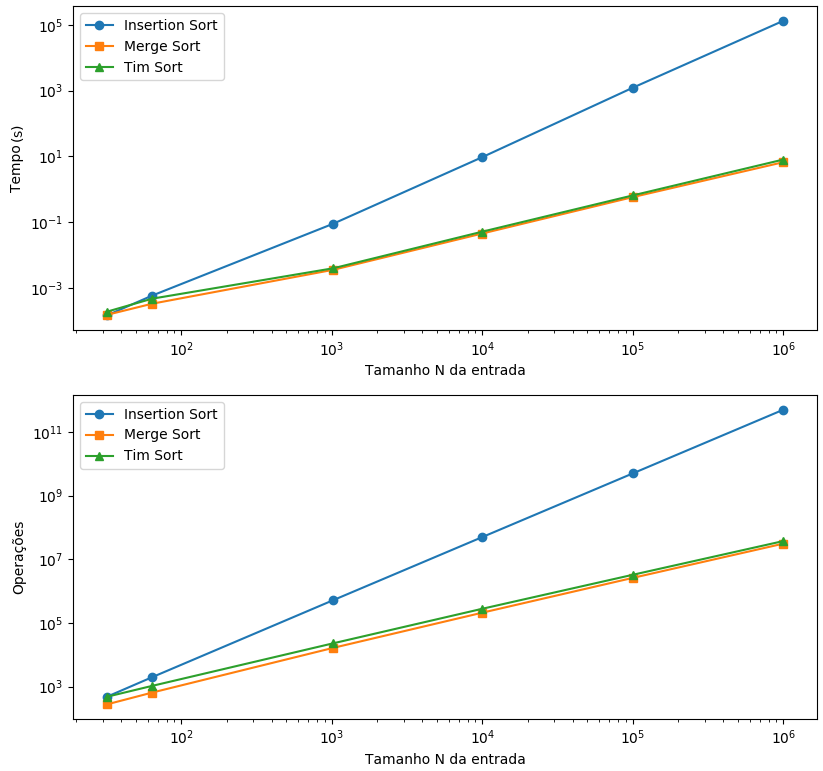
\includegraphics[width=15cm]{img/graficos_desc.png}
\caption{Resultados de execução para entrada ordenada decrescentemente}
\label{fig:grafico_desc}
\end{figure}

Por fim, para análise separada dos algoritmos Tim e Merge Sort, que demonstraram uma significativa melhor performance, são apresentados abaixo os gráficos para entradas crescentes e decrescentes, respectivamente. O baixo tempo de execução de ambos mesmo para entradas com muitos elementos, tornam a diferença significativamente pequena. Conforme observado anteriormente, o Tim Sort leva vantagem da configuração pré-ordenada crescentemente do vetor, mas, mesmo no cenário inverso, tem performance bem próxima do Merge Sort. 

\begin{figure}[!htb]
\centering
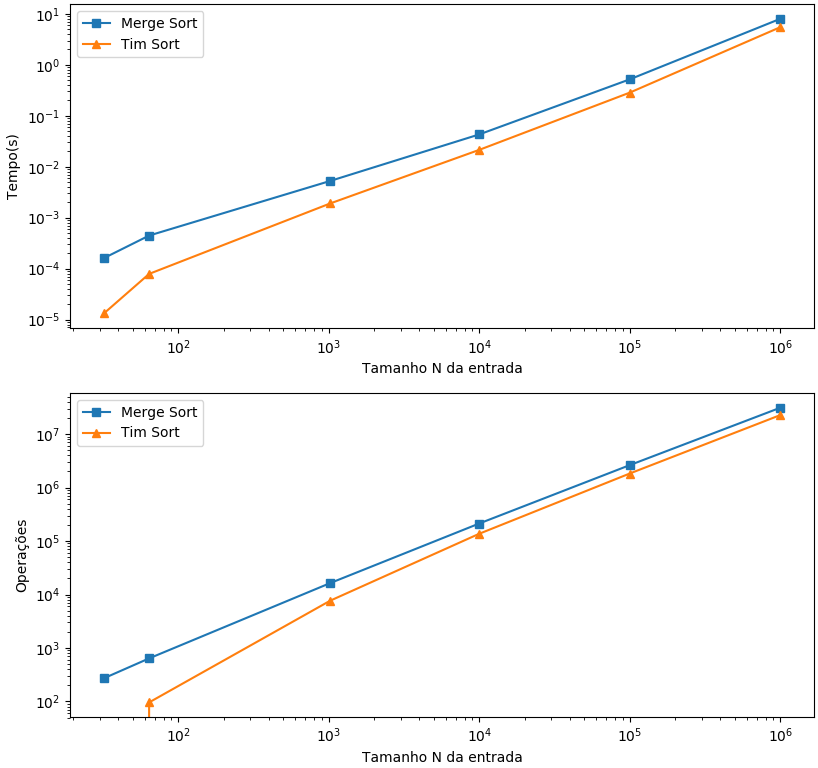
\includegraphics[width=15cm]{img/graficos_tim_merge.png}
\caption{Resultados de execução para entrada ordenada crescentemente}
\label{fig:grafico_tim_merge}
\end{figure}

\begin{figure}[!htb]
\centering
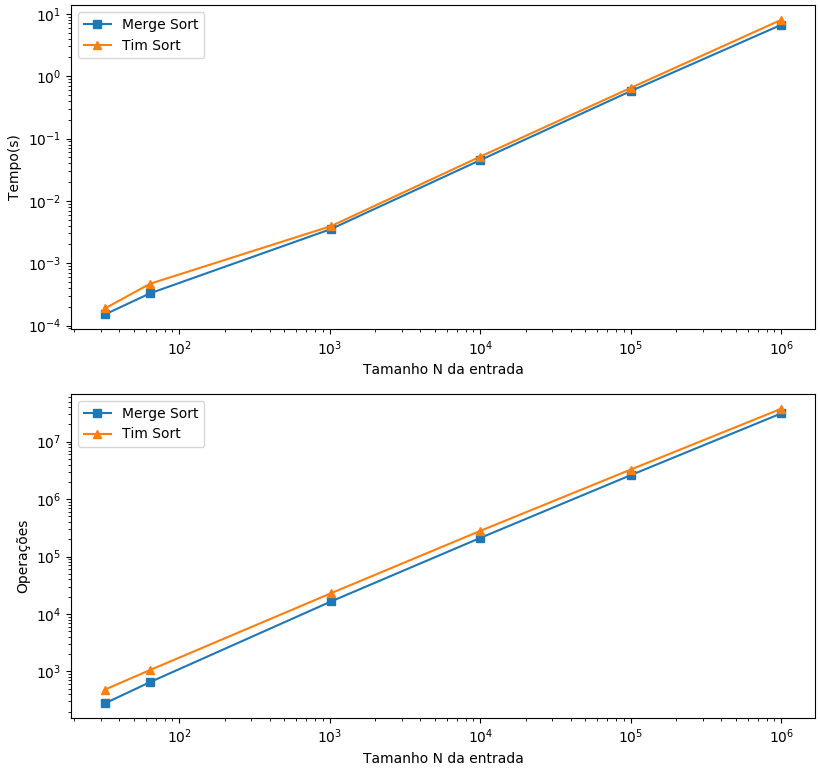
\includegraphics[width=15cm]{img/graficos_tim_merge2.png}
\caption{Resultados de execução para entrada ordenada decrescentemente}
\label{fig:grafico_tim_merge2}
\end{figure}

